\section{Aufgbau und Durchführung}
\label{sec:Durchführung}
\subsection{Aufbau}
Die Messaparatur ist aufgebaut wie in Abbildung \ref{fig:aufbau}.
\begin{figure}
  \centering
  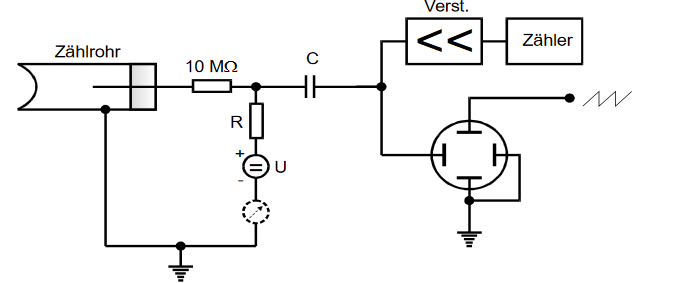
\includegraphics[width=0.6\textwidth]{aufbau.PNG}
  \caption{Aufbau der Messaparatur.}
  \label{fig:aufbau}
\end{figure}
Die im Zählrohr gesammelte Ladung fließt über den Widerstand $R$ ab und erzeugt einen Spannungsimpuls. Dieser wird über $C$ ausgekoppelt und
anschließend im Zähler registriert. Am Oszilloskop wird das Signal anschließend ausgegeben. Ein Beta-Strahler wird als Präparat
zur Messung genutzt.
\subsection{Durchführung}
Zu Begin wird die Charkteristik aufgenommen, dazu werden verschiedene Spannungen eingestellt und die Anzahl der entsprechenden
Impulse pro $10\si{\second}$ aufgenommen. Zur Bestimmung der freigesetzten Ladungsmenge pro Teilchen, wird ebenfalls der entsprechende
Strom $I$ notiert.
Qualitativ werden die Nachentladungen auf dem Oszilloskop sichtbar gemacht. Die Spannung wird auf das Maximum gesetzt. Gemessen
wird der zeitliche Abstand von Primär-und Nachladungsimpuls. Die Totzeit lässt sich am selben
Oszillogramm gemäß Abbildung \ref{fig:tz} abmessen.
Für die Bestimmung der Totzeit mit der Zwei-Quellen-Methode werden zwei Präparate genutzt. Zuerst wird die Zählrate
des ersten Präparates aufgenommen, dann das Zweite hinzugefügt und die Zählrate der beiden gemessen. Die Zählrate nur des zweiten Präparates
wird anschließend registriert.
